\documentclass[11pt]{article}

\usepackage[margin=1in]{geometry}
\usepackage{amsmath,amssymb}
\usepackage{bm}
\usepackage{enumitem}
\usepackage{hyperref}
\usepackage{tikz}
\usetikzlibrary{arrows.meta}

\newcommand{\vv}{\vec{v}}
\newcommand{\vx}{\vec{x}}
\newcommand{\vf}{\vec{f}}
\newcommand{\vb}{\vec{b}}
\newcommand{\vg}{\vec{g}}
\newcommand{\DDt}{\dfrac{D}{Dt}}

\title{Theoretical Foundations of Computational Fluid Dynamics\\
\large A Didactic Summary}
\author{Prepared as an introduction to the adhesive flow (shear-thinning) simulation project}
\date{}

\begin{document}
\maketitle

\section*{Purpose of this Summary}

Before simulating the flow of an adhesive with a shear-rate-dependent (shear-thinning) viscosity, it is worth reviewing where the governing equations of fluid dynamics come from and how they are solved numerically. This summary walks through that reasoning step by step, following the same logical path used to derive the incompressible Navier--Stokes equations and the finite volume method that discretizes them. The final section connects this foundation to the present project, where the constant-viscosity assumption used here is replaced by a shear-thinning constitutive law.

\section{From a Single Particle to a Continuum}

Classical mechanics describes the motion of a point mass $m$ subject to a force $\vf$. Its trajectory $\vx(t)$ follows Newton's second law,
\begin{equation}
  \frac{\mathrm{d}\vec{p}}{\mathrm{d}t} = \vf(\vx,\vx',t), \qquad \vec{p} = m\vv, \qquad \vv = \vx' ,
\end{equation}
an ordinary differential equation that, given initial position and velocity, has a unique solution.

A liquid, however, is made of an enormous number of interacting molecules; tracking each one is neither feasible nor useful. Instead, fluid dynamics replaces the discrete collection of particles with a \emph{continuum} description: rather than positions of molecules, we describe the state of the liquid by a mass density field
\begin{equation}
  \rho(\vx,t) \quad \text{[kg/m}^3\text{]},
\end{equation}
so that the mass contained in an arbitrary volume $V$ at time $t$ is
\begin{equation}
  m(t) = \int_V \rho(\vx,t)\, \mathrm{d}^3x .
\end{equation}
This is the key conceptual step of the chapter: classical mechanics is not abandoned, it is applied to infinitesimal fluid parcels that move with a velocity field $\vv(\vx,t)$, rather than to a single rigid body.

\section{Conservation of Mass: the Continuity Equation}

Because the liquid may be in motion, the mass inside a fixed volume $V$ can change over time if matter flows across its boundary $\partial V$. The rate at which mass crosses a surface is captured by the mass current density
\begin{equation}
  \vec{j}(\vx,t) = \rho(\vx,t)\,\vv(\vx,t) \qquad \text{[kg/(m}^2\text{s)]}.
\end{equation}

Global mass conservation states that the mass in $V$ changes only through flux across its boundary,
\begin{equation}
  \frac{\mathrm{d}}{\mathrm{d}t}\int_V \rho\,\mathrm{d}^3x = -\oint_{\partial V} \vec{j}\cdot \mathrm{d}\vec{\sigma}.
\end{equation}
Applying the divergence theorem to the right-hand side and noting that the identity must hold for \emph{any} volume $V$, the integrands themselves must be equal, giving the differential form: the \textbf{continuity equation},
\begin{equation}
  \frac{\partial \rho}{\partial t} + \operatorname{div}(\rho\vv) = 0 .
  \label{eq:continuity}
\end{equation}
This is the first of two field equations $\rho$ and $\vv$ must satisfy; it encodes nothing more than "mass is neither created nor destroyed."

\section{Conservation of Momentum: the Cauchy Equation}

The second equation follows from Newton's law applied to an infinitesimally small fluid parcel of volume $V$ moving with the flow, so that its mass is $m = V\rho(\vx,t)$. Dividing Newton's law by $V$ introduces the force per unit volume, the \textbf{body force} $\vb$,
\begin{equation}
  \rho(\vx,t)\,\frac{\mathrm{d}}{\mathrm{d}t}\vv(\vx(t),t) = \vb(\vx,t).
\end{equation}

Because the parcel's position $\vx(t)$ itself depends on time, the chain rule produces both an explicit and an implicit (advective) time dependence,
\begin{equation}
  \frac{\mathrm{d}}{\mathrm{d}t}\vv(\vx(t),t) = \Big[\partial_t + \vv\cdot\nabla\Big]\vv \;\equiv\; \frac{D\vv}{Dt},
\end{equation}
which defines the \textbf{material derivative} $D/Dt$ — the rate of change experienced by an observer riding along with the fluid, rather than sitting at a fixed point in space. This is the crucial conceptual device that turns a Lagrangian statement (Newton's law for a moving parcel) into an Eulerian field equation (evaluated at fixed points in space).

The body force $\vb$ is decomposed into external forces $\vf$ (e.g.\ gravity, $\vf = \rho\vg$) and internal, material-dependent forces arising from molecular interactions. These internal forces are collected into the \textbf{stress tensor} $\sigma$, a $3\times 3$ field
\begin{equation}
  \sigma =
  \begin{pmatrix}
    \sigma_{xx} & \tau_{xy} & \tau_{xz}\\
    \tau_{yx} & \sigma_{yy} & \tau_{yz}\\
    \tau_{zx} & \tau_{zy} & \sigma_{zz}
  \end{pmatrix},
  \qquad \vb = \vf + \operatorname{div}(\sigma).
\end{equation}

It is natural to further split $\sigma$ into an isotropic \textbf{pressure} contribution and a \textbf{stress deviator tensor} $\tau$ that captures viscous (frictional) effects:
\begin{equation}
  \sigma = -p\,\mathbf{I} + \tau ,
\end{equation}
where $\mathbf{I}$ is the identity tensor. Substituting this decomposition yields the most general form of the fluid dynamics equations, valid for any fluid:
\begin{align}
  \frac{\partial \rho}{\partial t} + \operatorname{div}(\rho\vv) &= 0, \label{eq:cont2}\\
  \rho\,\DDt\vv &= -\operatorname{grad}(p) + \operatorname{div}(\tau) + \rho\vg. \label{eq:cauchy}
\end{align}
Equation~\eqref{eq:cauchy} is the \textbf{Cauchy momentum equation}. At this stage the system is not yet closed: the pressure's dependence on $\rho$ and the stress deviator's dependence on the flow ($\tau(\rho,\vv)$) are still unspecified. These missing relations are the \textbf{constitutive equations}, and it is precisely at this point that different materials — Newtonian or non-Newtonian — part ways.

\section{Newtonian Fluids and the Navier--Stokes Equations}

The classical closure, due to Newton, restricts the functional form of $\tau$ by three physical assumptions:
\begin{enumerate}[label=(\roman*)]
  \item the fluid is isotropic (no preferred direction),
  \item no stress acts when the fluid is at rest ($\tau = 0$ when $\vv = 0$),
  \item $\tau$ is a \emph{linear} function of the velocity gradient.
\end{enumerate}
Under these assumptions the deviatoric stress must take the form
\begin{equation}
  \tau_{ij} = \mu\left(\frac{\partial v_i}{\partial x_j} + \frac{\partial v_j}{\partial x_i}\right) + \lambda\,\delta_{ij}\sum_{k=1}^{3}\frac{\partial v_k}{\partial x_k},
  \label{eq:newtonian-stress}
\end{equation}
where $\mu$ is the (first) coefficient of viscosity and $\lambda$ the second coefficient of viscosity. Crucially, $\mu$ is here a single \emph{constant} material property — the same at every point, independent of how fast the fluid is being sheared. Substituting Eq.~\eqref{eq:newtonian-stress} into the Cauchy equation gives the (compressible) \textbf{Navier--Stokes equations},
\begin{align}
  \frac{\partial \rho}{\partial t} + \operatorname{div}(\rho\vv) &= 0,\\
  \rho\,\DDt\vv &= -\operatorname{grad}(p) + \operatorname{div}\!\big[\mu\big(\operatorname{grad}(\vv)+\operatorname{grad}(\vv)^\top\big)\big] + \operatorname{div}\big[\lambda\operatorname{div}(\vv)\mathbf{I}\big] + \rho\vg.
\end{align}
One constitutive relation is still open: how $p$ depends on $\rho$ and $\vv$ (the equation of state).

\medskip
\noindent\textit{Where non-Newtonian fluids enter.} It is exactly assumption (iii) above — linearity of $\tau$ in the velocity gradient, with a constant $\mu$ — that a shear-thinning fluid violates. Section~\ref{sec:shear-thinning} revisits this closure without that assumption and derives the governing equations actually solved in the project code.

\section{Incompressible Newtonian Flow}

A very good approximation for most liquids (adhesives included, away from extreme pressures) is \textbf{incompressibility}: the density of a fluid parcel does not change as it moves with the flow, $D\rho/Dt = 0$. Combined with the continuity equation~\eqref{eq:cont2}, this forces the velocity field to be \textbf{divergence free},
\begin{equation}
  \operatorname{div}(\vv) = 0.
  \label{eq:divfree}
\end{equation}
This single kinematic constraint has two important consequences. First, it eliminates the $\lambda$ term from the momentum equation entirely. Second, it allows the viscous term to be simplified using the vector Laplacian, so that the governing system reduces to
\begin{align}
  \operatorname{div}(\vv) &= 0, \label{eq:incomp1}\\
  \rho\,\DDt\vv &= -\operatorname{grad}(p) + \mu\,\Delta\vv + \rho\vg. \label{eq:incomp2}
\end{align}
No equation of state is needed anymore: instead, the pressure field must be found such that it enforces Eq.~\eqref{eq:incomp1} at every instant. This is the system that will be solved numerically, and — with $\mu$ replaced by a shear-rate-dependent viscosity — is also the system underlying the present adhesive-flow project.

For completeness, the chapter also notes the further idealization of \textbf{inviscid, incompressible, constant-density} flow, which recovers the Euler equations
\begin{equation}
  \operatorname{div}(\vv) = 0, \qquad \DDt\vv = -\operatorname{grad}(w) + \vg, \qquad w \equiv p/\rho_0,
\end{equation}
useful for laminar flows but unable to capture viscous or turbulent effects — and therefore not the right model once viscosity (let alone shear-thinning viscosity) is the object of interest.

\section{Rheological Foundations and Governing Equations for Shear-Thinning Flow}
\label{sec:shear-thinning}

Accurate rheological modeling is the prerequisite for a predictive simulation. The Newtonian assumption of Sections~4--5 — a viscosity that is a fixed material constant — fails for the adhesive this project simulates, just as it fails for polymer melts, paints, and most other complex industrial fluids: their resistance to flow drops as they are sheared harder. Capturing this \textbf{shear-thinning} behavior, where viscosity is a dynamic function of the local shear rate rather than a constant, is essential for predicting how the adhesive actually dispenses and spreads.

\subsection{The Power-Law (Ostwald--de Waele) Model}

The most direct way to capture shear-thinning behavior is the \textbf{power-law model}. For the simple shear flow $u=u(y)$ shown in Fig.~\ref{fig:powerlaw} (flow in a single direction, varying only across the gap between two plates), it relates the shear stress $\tau_{yx}$ to the shear rate $\mathrm{d}u/\mathrm{d}y$ by
\begin{equation}
  \tau_{yx} = K\left(\frac{\mathrm{d}u}{\mathrm{d}y}\right)^{n},
  \label{eq:powerlaw-1d}
\end{equation}
where $K$ is the \textbf{consistency index} (the fluid's overall resistance to flow) and $n$ is the \textbf{flow behavior index}. When $n<1$ the fluid is \textbf{pseudoplastic} (shear-thinning); when $n>1$ it is \textbf{dilatant} (shear-thickening); $n=1$ recovers the Newtonian fluid with $K=\mu$, the straight line in the figure.

\begin{figure}[htbp]
\centering
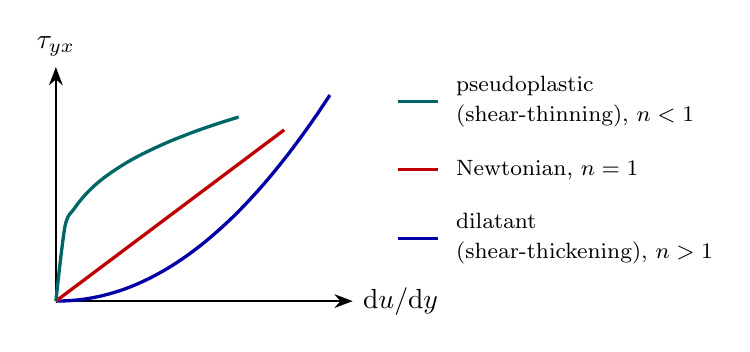
\begin{tikzpicture}[scale=1.45, >=Stealth]
% axes
\draw[->, thick] (0,0) -- (2.6,0) node[right] {$\mathrm{d}u/\mathrm{d}y$};
\draw[->, thick] (0,0) -- (0,2.05) node[above] {$\tau_{yx}$};

% dilatant (shear-thickening), convex, blue, n>1
\draw[very thick, blue!65!black, smooth]
  plot coordinates {(0.000,0.000) (0.120,0.004) (0.240,0.016) (0.360,0.037)
  (0.480,0.067) (0.600,0.105) (0.720,0.153) (0.840,0.210) (0.960,0.276)
  (1.080,0.351) (1.200,0.436) (1.320,0.530) (1.440,0.634) (1.560,0.746)
  (1.680,0.869) (1.800,1.001) (1.920,1.143) (2.040,1.294) (2.160,1.455)
  (2.280,1.625) (2.400,1.805)};

% Newtonian, straight, red
\draw[very thick, red!75!black] (0,0) -- (2.0,1.5);

% pseudoplastic (shear-thinning), concave, teal, n<1
\draw[very thick, teal!80!black, smooth]
  plot coordinates {(0.000,0.000) (0.080,0.656) (0.160,0.808) (0.240,0.912)
  (0.320,0.995) (0.400,1.064) (0.480,1.123) (0.560,1.176) (0.640,1.225)
  (0.720,1.269) (0.800,1.309) (0.880,1.347) (0.960,1.383) (1.040,1.417)
  (1.120,1.448) (1.200,1.479) (1.280,1.508) (1.360,1.535) (1.440,1.562)
  (1.520,1.587) (1.600,1.612)};

% ---- legend, to the right of the axes ----
\draw[very thick, teal!80!black] (3.0,1.75) -- (3.35,1.75);
\node[anchor=west, align=left] at (3.42,1.75) {\footnotesize pseudoplastic\\[-1pt]\footnotesize(shear-thinning), $n<1$};

\draw[very thick, red!75!black] (3.0,1.15) -- (3.35,1.15);
\node[anchor=west] at (3.42,1.15) {\footnotesize Newtonian, $n=1$};

\draw[very thick, blue!65!black] (3.0,0.55) -- (3.35,0.55);
\node[anchor=west, align=left] at (3.42,0.55) {\footnotesize dilatant\\[-1pt]\footnotesize(shear-thickening), $n>1$};

\end{tikzpicture}
\caption{Shear stress versus shear rate for simple shear flow $u=u(y)$. The Newtonian fluid gives a straight line through the origin. Pseudoplastic (shear-thinning) fluids give a concave curve -- the apparent viscosity, the local slope $\tau_{yx}/(\mathrm{d}u/\mathrm{d}y)$, decreases as the shear rate grows. Dilatant (shear-thickening) fluids give a convex curve, with an apparent viscosity that instead increases. All three are special cases of the power law, Eq.~\eqref{eq:powerlaw-1d}, with flow behavior index $n<1$, $n=1$, and $n>1$ respectively.}
\label{fig:powerlaw}
\end{figure}

Dividing Eq.~\eqref{eq:powerlaw-1d} by the shear rate gives the \textbf{apparent viscosity} $\eta = K|\dot\gamma|^{\,n-1}$, where $\dot\gamma\equiv\mathrm{d}u/\mathrm{d}y$. This is where the model's one real weakness shows up: for a pseudoplastic fluid ($n<1$), $\eta\to\infty$ as $\dot\gamma\to0$. Physically nothing is wrong -- the true stress $\tau_{yx}=K\dot\gamma^n$ stays perfectly finite, and in fact vanishes, as $\dot\gamma\to0$ -- but the apparent-viscosity form the code actually has to evaluate blows up, and $\dot\gamma\approx0$ is not a rare corner case: it occurs at every symmetry plane and channel centerline, exactly where the solver needs $\eta$ at every iteration. The standard fix is to regularize the shear rate before raising it to the $n-1$ power,
\begin{equation}
  \dot\gamma_{\mathrm{eff}} = \sqrt{\dot\gamma^2+\varepsilon^2},
  \label{eq:reg-1d}
\end{equation}
with $\varepsilon$ a small constant well below the smallest shear rate of physical interest in the flow.

\subsection{From a Single Shear Component to the Full Tensor}

Equation~\eqref{eq:powerlaw-1d} is only valid for the simple shear flow $u=u(y)$, where the fluid slides in a single direction. The flows this project simulates are two-dimensional, with both velocity components $v_x$ and $v_y$ varying in both $x$ and $y$, so the single number $\mathrm{d}u/\mathrm{d}y$ must be replaced by a quantity that captures the local rate of deformation in every direction at once: the \textbf{rate-of-strain tensor} $\mathbf{D}$, the symmetric part of the velocity gradient,
\begin{equation}
  \mathbf{D} \equiv \tfrac{1}{2}\big(\operatorname{grad}(\vv) + \operatorname{grad}(\vv)^\top\big), \qquad D_{ij} = \tfrac{1}{2}\left(\frac{\partial v_i}{\partial x_j}+\frac{\partial v_j}{\partial x_i}\right).
  \label{eq:strain-rate}
\end{equation}
Only the symmetric part matters: the remaining antisymmetric part of the velocity gradient is a pure local rotation, and a rotating fluid element slides past none of its neighbors, so an isotropic fluid generates no stress from it. Figure~\ref{fig:strain-rotation} illustrates the split.

\begin{figure}[htbp]
\centering
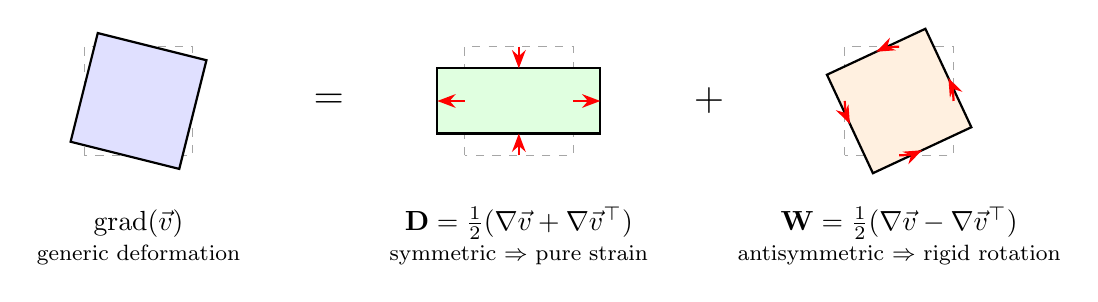
\begin{tikzpicture}[scale=1.15, >=Stealth]

% ---------- Panel 1: generic velocity gradient (deformation + rotation) ----------
\begin{scope}[xshift=0cm]
  \draw[dashed, gray!70] (-0.6,-0.6) rectangle (0.6,0.6);
  \draw[thick, fill=blue!12]
    (-0.75,-0.45) -- (0.45,-0.75) -- (0.75,0.45) -- (-0.45,0.75) -- cycle;
  \node at (0,-1.35) {$\operatorname{grad}(\vv)$};
  \node at (0,-1.7) {\footnotesize generic deformation};
\end{scope}

\node at (2.1,0) {\Large $=$};

% ---------- Panel 2: symmetric part D (pure strain) ----------
\begin{scope}[xshift=4.2cm]
  \draw[dashed, gray!70] (-0.6,-0.6) rectangle (0.6,0.6);
  \draw[thick, fill=green!12] (-0.9,-0.36) rectangle (0.9,0.36);
  \draw[->, red, thick] (0.6,0)  -- (0.9,0);
  \draw[->, red, thick] (-0.6,0) -- (-0.9,0);
  \draw[->, red, thick] (0,0.6)  -- (0,0.36);
  \draw[->, red, thick] (0,-0.6) -- (0,-0.36);
  \node at (0,-1.35) {$\mathbf D=\tfrac12(\nabla\vv+\nabla\vv^\top)$};
  \node at (0,-1.7) {\footnotesize symmetric $\Rightarrow$ pure strain};
\end{scope}

\node at (6.3,0) {\Large $+$};

% ---------- Panel 3: antisymmetric part W (rigid rotation) ----------
\begin{scope}[xshift=8.4cm]
  \draw[dashed, gray!70] (-0.6,-0.6) rectangle (0.6,0.6);
  \draw[thick, fill=orange!12]
    (-0.2898,-0.7974) -- (0.7974,-0.2898) -- (0.2898,0.7974) -- (-0.7974,0.2898) -- cycle;
  \draw[->, red, thick] (0.6,0)   arc[start angle=0, end angle=25, radius=0.6];
  \draw[->, red, thick] (0,0.6)   arc[start angle=90, end angle=115, radius=0.6];
  \draw[->, red, thick] (-0.6,0)  arc[start angle=180, end angle=205, radius=0.6];
  \draw[->, red, thick] (0,-0.6)  arc[start angle=270, end angle=295, radius=0.6];
  \node at (0,-1.35) {$\mathbf W=\tfrac12(\nabla\vv-\nabla\vv^\top)$};
  \node at (0,-1.7) {\footnotesize antisymmetric $\Rightarrow$ rigid rotation};
\end{scope}

\end{tikzpicture}
\caption{Decomposition of the local velocity gradient acting on a small fluid element (dashed square = undeformed element; the three panels are drawn schematically, with exaggerated magnitudes, to illustrate the \emph{character} of each contribution rather than an exact geometric sum). The symmetric part $\mathbf D$ stretches and shears the element: neighboring fluid particles move relative to one another, and it is exactly this relative sliding that a viscous stress resists. The antisymmetric part $\mathbf W$ merely spins the element as a rigid body: every particle keeps the same distance and orientation relative to its neighbors, so there is no relative motion for viscosity to act on, and an isotropic fluid generates no stress from it.}
\label{fig:strain-rotation}
\end{figure}

Comparing Eq.~\eqref{eq:strain-rate} with the Newtonian stress relation, Eq.~\eqref{eq:newtonian-stress}, shows that the Newtonian case is simply $\tau=2\mu\mathbf{D}+\lambda\operatorname{tr}(\mathbf{D})\mathbf{I}$, which for an incompressible fluid ($\operatorname{div}(\vv)=0\Rightarrow\operatorname{tr}(\mathbf{D})=0$) reduces to the compact form
\begin{equation}
  \tau = 2\mu\,\mathbf{D}.
  \label{eq:tau-newtonian-compact}
\end{equation}
A \textbf{generalized Newtonian fluid} keeps this same form — stress proportional to the rate of strain — but lets the proportionality "constant" depend on the flow itself through the scalar magnitude of $\mathbf{D}$,
\begin{equation}
  \tau = 2\,\eta(|\mathbf{D}|)\,\mathbf{D}, \qquad |\mathbf{D}| \equiv \sqrt{\mathbf{D}:\mathbf{D}} = \sqrt{D_{xx}^2+D_{yy}^2+2D_{xy}^2}\quad\text{(2D)}.
  \label{eq:generalized-newtonian}
\end{equation}
This is the direct tensor generalization of the power law: identifying $\eta(|\mathbf{D}|)$ with $K\,|\mathbf{D}|^{\,n-1}$ recovers Eq.~\eqref{eq:powerlaw-1d} for the simple shear flow, and regularizing it exactly as in Eq.~\eqref{eq:reg-1d},
\begin{equation}
  \eta(|\mathbf{D}|) = K\,D_{\mathrm{eff}}^{\,n-1}, \qquad D_{\mathrm{eff}} \equiv \sqrt{|\mathbf{D}|^2 + \varepsilon^2},
  \label{eq:powerlaw-regularized}
\end{equation}
\begin{sloppypar}
is exactly what the code's \texttt{compute\_shear\_and\_viscosity()} step evaluates: \texttt{D\_eff = sqrt(Dmag*Dmag + POWERLAW\_EPSILON * POWERLAW\_EPSILON)}, followed by \texttt{eta = POWERLAW\_K * pow(D\_eff, POWERLAW\_N - 1.0)}. (One bookkeeping note: the code's $|\mathbf{D}|=\sqrt{\mathbf{D}:\mathbf{D}}$ differs by a constant factor $\sqrt2$ from the shear-rate invariant $\dot\gamma\equiv\sqrt{2\,\mathbf{D}:\mathbf{D}}$ used in some rheology references; that factor is absorbed into $K$ and does not change the physics.) Setting $n=1$ recovers the constant-viscosity Newtonian stress $\tau=2\mu\mathbf{D}$, with $K$ playing the role of $\mu$ — the same consistency check as in the 1D picture.
\end{sloppypar}

\subsection{Governing Equations}

Substituting Eq.~\eqref{eq:generalized-newtonian} into the incompressible Cauchy equation gives the two equations the code solves,
\begin{align}
  \operatorname{div}(\vv) &= 0, \label{eq:st-continuity}\\
  \rho\,\DDt\vv &= -\operatorname{grad}(p) + \operatorname{div}\!\big(2\,\eta(|\mathbf{D}|)\,\mathbf{D}\big) + \rho\vg. \label{eq:st-momentum}
\end{align}
Mass conservation is untouched; the only change from the Newtonian case, Eqs.~\eqref{eq:incomp1}--\eqref{eq:incomp2}, is that the constant $\mu$ inside the viscous term has become the field $\eta(|\mathbf{D}(\vx,t)|)$, evaluated with the regularized power law of Eq.~\eqref{eq:powerlaw-regularized}.

Physically, this produces a \textbf{plug-flow} velocity profile. Because $\eta$ is lowest where the shear is highest — right at the walls — the fluid slides more easily there, while the core of the channel, where shear is weak, keeps a high viscosity and moves together almost as a solid plug, instead of the smooth parabola of Newtonian (Poiseuille) flow. For an adhesive being dispensed through a nozzle, this is a direct practical payoff: the same driving pressure pushes more material through, since the low near-wall viscosity does most of the work of overcoming friction against the walls.

\subsection{Consequences for the Viscous Term}

In Section~5, incompressibility allowed the viscous term to be simplified from $\operatorname{div}[\mu(\operatorname{grad}(\vv)+\operatorname{grad}(\vv)^\top)]$ down to the vector Laplacian $\mu\,\Delta\vv$, by pulling the \emph{constant} $\mu$ out of the divergence and using $\operatorname{div}(\vv)=0$. With $\eta$ now a field that varies from cell to cell through $|\mathbf{D}(\vx,t)|$, it can no longer be taken outside the divergence: $\operatorname{div}(2\eta\mathbf{D}) \neq \eta\,\Delta\vv$ in general. The momentum equation must therefore be discretized keeping the \emph{full stress divergence} of Eq.~\eqref{eq:st-momentum}, evaluated component-wise — precisely what is implemented in the code, where the viscous contribution to each velocity component is built from face-averaged viscosities $\eta_e,\eta_w,\eta_n,\eta_s$ acting on the corresponding stress components, rather than from a simple five-point Laplacian stencil.

A further consequence, worth flagging explicitly, concerns the pressure Poisson equation of Section~\ref{sec:pressure-poisson}: its derivation there also relies on $\mu$ being constant (to interchange derivatives and cancel the mixed terms). With $\eta$ spatially varying, an exact source term would carry additional contributions involving $\operatorname{grad}(\eta)$. The current implementation retains the constant-viscosity Poisson source as a documented simplification, deferring the fully consistent variable-viscosity pressure correction to future work.

\section{Discretization: the Finite Volume Method}

Equations~\eqref{eq:incomp1}--\eqref{eq:incomp2} are nonlinear PDEs and must, in general, be solved numerically. The chapter develops the \textbf{finite volume method} (FVM), which is the natural discretization for conservation laws because it works directly with integrated fluxes rather than pointwise derivatives.

\subsection{Control Volumes and the Integrated Momentum Equation}

Space is subdivided into small control volumes (cuboids of size $\Delta_x\times\Delta_y\times\Delta_z$), each with a control point $\vec c$ — conventionally its center — at which the field values $(p,\vv)$ are stored. Integrating the $k$-th component of the momentum equation over one such volume $V$ and using $\partial_k p = \operatorname{div}(p\,\vec e_k)$ turns every volume integral of a divergence into a surface integral via the Gauss theorem:
\begin{equation}
  \frac{\partial}{\partial t}\int_V v_k\,\mathrm{d}^3x + \int_V \vv\cdot\operatorname{grad}(v_k)\,\mathrm{d}^3x
  = -\frac{1}{\rho_0}\oint_{\partial V} p\,\vec e_k\cdot\mathrm{d}\vec\sigma + \frac{\mu}{\rho_0}\oint_{\partial V}\operatorname{grad}(v_k)\cdot\mathrm{d}\vec\sigma + \int_V g_k\,\mathrm{d}^3x.
\end{equation}

\subsection{Volume and Surface Integrals}

At leading order, a volume integral is approximated by the value at the control point times the cell volume,
\begin{equation}
  \int_V f(\vx)\,\mathrm{d}^3x = f(\vec c)\,\Delta_x\Delta_y\Delta_z + O(\Delta^2),
\end{equation}
while a surface integral over, e.g., the east face is approximated by the value at the face center times the face area,
\begin{equation}
  \int_e \vf(\vx)\cdot\mathrm{d}\vec\sigma = \Delta_y\Delta_z\,f_x(\vec e) + O(\Delta^2).
\end{equation}
Field values not stored directly at control points (face centers, edges, corners) are obtained by interpolation — e.g., Lagrange polynomials fitted through neighboring control points.

A defining feature of the FVM, and the reason it is the method of choice for fluid dynamics, is that two neighboring cells $V_1,V_2$ share a common face, so the surface integral computed there is identical (up to sign) for both cells,
\begin{equation}
  \int_{e_1} \vf\cdot\mathrm{d}\vec\sigma = -\int_{w_2} \vf\cdot\mathrm{d}\vec\sigma .
\end{equation}
When this flux is evaluated only once numerically and shared between the two cells, whatever leaves $V_1$ through that face exactly enters $V_2$: the discrete scheme is \textbf{conservative by construction}, even in the presence of numerical error in the flux value itself.

\subsection{The Leading-Order 2D Scheme}

Restricting to two dimensions and using simple central differences for the spatial derivatives at the control point and its four neighbors (east $\vec E$, west $\vec W$, north $\vec N$, south $\vec S$), the momentum equation becomes an explicit update rule,
\begin{align}
  v_k(\vec c, t+\Delta_t) = {} & v_k(\vec c,t) + \Delta_t\Bigg[g_k(\vec c,t)\notag\\
  & - v_x(\vec c,t)\frac{v_k(\vec e,t)-v_k(\vec w,t)}{\Delta_x} - v_y(\vec c,t)\frac{v_k(\vec n,t)-v_k(\vec s,t)}{\Delta_y}\notag\\
  & -\frac{1}{\rho_0}\Big(\frac{p(\vec e,t)-p(\vec w,t)}{\Delta_x}\delta_{kx} + \frac{p(\vec n,t)-p(\vec s,t)}{\Delta_y}\delta_{ky}\Big)\notag\\
  & + \frac{\mu}{\rho_0}\,\frac{1}{\Delta_x}\left(\frac{v_k(\vec E,t)-v_k(\vec c,t)}{\|\vec E-\vec c\|} - \frac{v_k(\vec c,t)-v_k(\vec W,t)}{\|\vec c-\vec W\|}\right)\notag\\
  & + \frac{\mu}{\rho_0}\,\frac{1}{\Delta_y}\left(\frac{v_k(\vec N,t)-v_k(\vec c,t)}{\|\vec N-\vec c\|} - \frac{v_k(\vec c,t)-v_k(\vec S,t)}{\|\vec c-\vec S\|}\right)\Bigg].
\end{align}
Two observations are worth keeping in mind: on a regular grid, this lowest-order finite volume scheme coincides exactly with a finite difference scheme; and this equivalence breaks down at higher order or on irregular geometries, which is where the finite volume viewpoint (fluxes through faces) becomes genuinely more powerful than a naive finite-difference stencil.

\subsection{The Pressure Poisson Equation}
\label{sec:pressure-poisson}

Because density is constant, no equation of state closes the system — instead, the pressure must be chosen at every time step so that the resulting velocity field stays divergence-free. Taking the divergence of the momentum equation and using incompressibility to eliminate the mixed derivative terms yields a \textbf{Poisson equation} for the pressure,
\begin{equation}
  \Delta p = \rho_0\operatorname{div}(\vg) - \rho_0\Big[(\partial_x v_x)^2 + (\partial_y v_y)^2 + 2(\partial_x v_y)(\partial_y v_x)\Big].
  \label{eq:poisson}
\end{equation}
This is a \emph{linear} elliptic equation (unlike the nonlinear momentum equation) and can be solved with any standard method once the velocity field is known. Only $\operatorname{grad}(p)$ enters the dynamics, so the pressure is determined up to an additive constant.

Discretizing Eq.~\eqref{eq:poisson} at each control point gives a large linear system, one equation per interior cell. The chapter solves it with the \textbf{Jacobi iteration}: starting from a guess, every cell's pressure is updated from its four neighbors, this sweep is repeated over all cells, and the whole process is iterated until the change between successive iterates falls below a chosen tolerance.

\subsection{Time Stepping and Boundary Conditions}

Combining the two ingredients gives the overall explicit algorithm advancing from time $t$ to $t+\Delta_t$:
\begin{enumerate}[label=\arabic*.]
  \item \textbf{Evolve the velocities} using the momentum equation with the pressure at time $t$.
  \item \textbf{Update the pressure} by solving the Poisson equation~\eqref{eq:poisson} with the newly evolved velocity field.
\end{enumerate}
This scheme has an error of $O(\Delta_t^2)$ per step; a higher-order time derivative would reduce this error but requires solving the (nonlinear) momentum equation implicitly.

For the problem to be well posed, the system needs an initial condition $\vv(\vx,0)=\vv_0$ with $\operatorname{div}(\vv_0)=0$, and a boundary condition on $\partial\Omega$. The chapter discusses:
\begin{itemize}
  \item \textbf{Dirichlet conditions}, $\vv(\vx,t) = \vv_b(\vx,t)$ on the boundary; the special case $\vv_b = 0$ is the \textbf{no-slip} condition (fluid sticks to a solid wall) — the natural condition at the walls of an adhesive-flow geometry.
  \item \textbf{Free-slip conditions}, where only the normal component $\vec n\cdot\vv = 0$ is enforced.
  \item A consistent \textbf{Neumann condition} for the pressure, derived from the velocity field at the boundary, often approximated in practice by $\vec n\cdot\operatorname{grad}(p) = 0$ (at the cost of slowly degrading the divergence-free property over time).
\end{itemize}

\section*{From this Chapter to the Project}

This chapter builds the machinery in two stages: first the incompressible Navier--Stokes equations, Eqs.~\eqref{eq:incomp1}--\eqref{eq:incomp2}, under the Newtonian assumption of a single constant viscosity $\mu$; then, in Section~\ref{sec:shear-thinning}, their shear-thinning generalization, Eqs.~\eqref{eq:st-continuity}--\eqref{eq:st-momentum} with the regularized power-law closure of Eq.~\eqref{eq:powerlaw-regularized}, which is the model actually solved by the project code. Mass conservation, the Cauchy momentum balance, the incompressibility constraint, and the finite-volume discretization strategy — control volumes, flux-conservative face integrals, the explicit velocity update, and the pressure Poisson equation — all carry over unchanged between the two stages. What changes is only the constitutive law that fixes $\tau$: the viscous term $\operatorname{div}(\tau)$ must now be evaluated as a full stress divergence with a viscosity that depends on the locally computed rate of strain, rather than being pulled outside the divergence as a constant $\mu\Delta\vv$. This is the theoretical starting point developed in the remainder of the report.

\end{document}
